\documentclass[11pt,a4paper]{article}

\usepackage[polish]{babel}
\usepackage[utf8]{inputenc}
\usepackage{polski}
\usepackage[T1]{fontenc}
\usepackage{indentfirst}
\usepackage{wrapfig}    % for wrapping figures, tables

\frenchspacing

%\usepackage{amsmath}
\usepackage{physics}
%\usepackage{bm}
\usepackage{gensymb}
%\usepackage{hepnames}
\usepackage{epsfig}
\usepackage{graphics}
\usepackage[shortlabels]{enumitem}
%\usepackage{xspace}
%\xspaceaddexceptions{[]\{\}}

%
%
%fixpagesize
\pagestyle{empty}
\addtolength{\textwidth}{6cm}
\addtolength{\textheight}{4cm}
\addtolength{\evensidemargin}{-3cm}
\addtolength{\oddsidemargin}{-3cm}
\addtolength{\topmargin}{-2cm}
\parindent=0cm

%
%
%small distance in list/item/enum for enumitem package
\setlist[itemize,enumerate]{topsep=0em}
\setlist{noitemsep}


% definition of inexact differential symbol:
\newcommand{\dbar} {\ensuremath{\,\mathchar'26\mkern-12mu d}}

%print zadanie #
\newcounter{zadanie}\newcommand{\zadanie}[1][]{\addtocounter{zadanie}{1} ~\\  {\bf \emph{Zadanie \arabic{zadanie} #1 }} \\}
\newcounter{zaddom}\newcommand{\zaddom}[1][]{\addtocounter{zaddom}{1} ~\\  {\bf \emph{Zadanie domowe \arabic{zaddom} #1 }} \\}
%\renewcommand{\zadanie}[1][]{\pagebreak  ~\\  {\bf \emph{Zadanie }} \\} \addtolength{\topmargin}{-2cm}


%
%%%%%%%%%%%%%%%%%%%%%%%%%%%%%%%%%%%%%%%%%%%%%%%%%%%%%%
% Changes figure placing algorithm
\renewcommand{\topfraction}{1}       % maximal fraction of a page allowed for figures
\renewcommand{\textfraction}{0.15}   % minimal number of text for figure-text shared pages
\renewcommand{\floatpagefraction}{0.95} % if two above does not help, this could do the job
                                        % must be: floatpagefraction < topfraction !!!!
%
\renewcommand{\textfraction}{0} % minimum fraction of page, which must be
                                % devoted to text
\renewcommand{\topfraction}{1}  % maximum fraction at top, which can be
                                % occupied whit floats
\setcounter{totalnumber}{400}   % increase the number of floats for one page
\setcounter{topnumber}{200}     % at all/top/bottom.
\setcounter{bottomnumber}{200}  %


\begin{document}           % End of preamble and beginning of text.
\begin{centering}

\vspace*{-1cm}

\bf{\Large{Termodynamika z elementami fizyki statystycznej}}\\
Tydzień 14 (8 czerwca 2023)\\[5mm]
napięcie powierzchniowe, transport ciepła\\
\end{centering} 

\vspace*{0mm}
\zadanie
Zakładając, że energia potencjalna związana z napięciem powierzchniowym jednostronnej błony cieczy jest
równa $E_p = \sigma \cdot S$, gdzie $S$ – powierzchnia, $\sigma$ – współczynnik napięcia
powierzchniowego, policzyć energię błony rozpiętej na długich prętach rozmieszczonych
w narożach kwadratu, jeśli:\\[1mm]
\hspace*{10ex} a) błona tworzy kształt:
\hspace*{20ex} b) błona tworzy kształt: \\
\hspace*{13ex}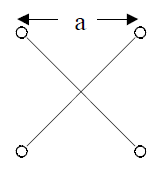
\includegraphics[width=22mm]{blona1.png}
\hspace*{32ex}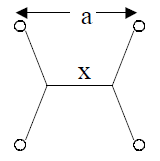
\includegraphics[width=22mm]{blona2.png}
\\
W którym przypadku energia jest mniejsza? Jakiej wartości $x$ odpowiadać będzie minimum energii?

\zadanie
Policzyć ciśnienie panujące wewnątrz bańki mydlanej o promieniu $r$.
Ile wynosi to ciśnienie dla $r = 1$\,mm? Przyjąć napięcie powierzchniowe takie,
jak dla wody $\sigma = 0.073$\,N/m.\\[1mm]
{\em Wskazówka: Porównać pracę potrzebną na powiększenie promienia bańki o $dr$
ze zmianą energii błony bańki.}

\zadanie
Szklaną kapilarę o wewnętrznym promieniu $R = 0.1$\,mm i długości $H = 20$\,cm wsunięto pionowo
do wody. Górny koniec rurki jest szczelnie zamknięty. Jaki odcinek $h$ kapilary należy zanurzyć,
aby poziom w rurce i na zewnątrz był jednakowy?
Przyjmij, że: ciśnienie powietrza $p_0 = 1020$\,hPa,
woda doskonale zwilża powierzchnię rurki (tzn. $\sigma=-\alpha$,
gdzie $\alpha$ jest współczynnikiem przylegania wody do szkła),
stała napięcia powierzchniowego wody $\sigma = 0.073$\,J/m$^2$,
oraz powietrze można traktować jako gaz doskonały.

\zadanie
Rozwiązać jednowymiarowe równanie transportu ciepła:
\[ \frac{\partial T}{\partial t} = \frac{\lambda}{\rho c}\cdot
                                   \frac{\partial^2 T}{\partial x^2} \]
metodą rozdzielania zmiennych, czyli zakładając, że rozwiązania
bazowe mają postać iloczynu:
\[ T(x,t) = X(x)\cdot{\displaystyle \tau}(t).\]

\zadanie
Pręt styka się na obu końcach z ciałami o temperaturze $T_1$.
W chwili początkowej rozkład temperatury w pręcie dany jest funkcją:
\[ T(x,t=0) \,=\, T_1 + A \cos^3 \left(\frac{\pi x}{L}\right), \]
gdzie $-L/2 < x < L/2$.
Jak zależy od czasu rozkład temperatury w pręcie?\\[1mm]
{\em Wskazówka: Skorzystać z równości
~$\cos{\alpha} = {1\over 2} (e^{i\alpha}+e^{-i\alpha})$.}

\zadanie
Znaleźć rozkład temperatury w gruncie w stanie ustalonym przy założeniu,
że grunt jest ośrodkiem jednorodnym o poziomej powierzchni oraz że
temperatura na powierzchni gruntu zmienia się zgodnie ze wzorem:
\[ T(x=0, y,z,t) \,=\, A \cos(\omega t) + T_\circ. \]

%%%%%%%%%%%%%%%%%%%%%%%%%%
\newpage
%%%%%%%%%%%%%%%%%%%%%%%%%%

\zaddom
Rurka barometryczna o średnicy wewnętrznego przekroju $d = 4\,$mm wypełniona jest rtęcią i zanurzona otwartym
końcem w szerokim naczyniu z rtęcią. Różnica poziomów rtęci w rurce i naczyniu wynosi $\Delta h = 756\,$mm.
Jakie jest ciśnienie atmosferyczne, jeżeli wiadomo, że rtęć jest cieczą całkowicie niezwilżającą (tzn. kąt zwilżania $\theta = \pi$) dla szkła?
Gęstość rtęci $\rho = 13.56\,{\rm g/cm^3}$, przyspieszenie ziemksie $g = 9.81$~m/s$^{2}$
Współczynnik napięcia powierzchniowego $\sigma = 0.47\,$N/m.

{\it Odpowiedź:} $(p-gh\rho) d/4=\sigma$ czyli $p=4\sigma/d+gh\rho\simeq 1009.8$hPa

\zaddom
Energia płynie od ciała o temperaturze $T_1 = 500\,$K do ciała o temperaturze
$T_2 = 300\,$K przez dwa „szeregowo” połączone pręty o tej samej długości i tym samym polu przekroju.
Pierwszy z prętów wykonany jest z miedzi ($\lambda_{Cu} = 400\,{\rm \frac{W}{m\cdot K}}$),
a drugi z żelaza ($\lambda_{Fe} = 50\,{\rm \frac{W}{m\cdot K}}$).
Jaka jest temperatura $T$ połączenia prętów?

{\it Odpowiedź:}
Temperatura rozkłada się liniowo, tj.
$T=(\lambda_{Cu} T_1+\lambda_{Fe} T_2)/(\lambda_{Cu}+\lambda_{Fe})=477$~K


\zaddom
Pręt styka się na obu końcach z ciałami o stałej temperaturze $T_1$.
W chwili początkowej rozkład temperatury w pręcie dany jest funkcją
$T(x,0) = T_1 + A\cdot \sin(x)+\frac{A}{2}\cdot \sin(2x)$, gdzie
$x\in [0, \pi]$. Jak zależy od czasu temperatura pręta?

{\it Odpowiedź:}
$T(x,t) = T_1 + Ae^{-\lambda t/\rho c}\cdot \sin(x)+\frac{A}{2}e^{-4\lambda t/\rho c}\cdot \sin(2x)$

% An example of figure placement:
%\begin{wrapfigure}[13]{r}{0.4\linewidth}\vspace{3mm}
%\resizebox{\linewidth}{!}{\includegraphics{NAZWA.png}}
%\end{wrapfigure}
%\zaddom

\end{document}

\zaddom
Do cieczy w szerokim poziomym naczyniu włożono pionowo cienką rurkę o wewnętrznym promieniu równym $r$.
Współczynnik napięcia powierzchniowego cieczy jest równy $\sigma$,
współczynnik przylegania cieczy do ciała stałego jest równy $\alpha$.
\begin{enumerate}
\item Jakie jest położenie górnego poziomu cieczy wewnątrz rurki?
      Wynik przedyskutować w funkcji współczynnika $\alpha$.
\item Na jaką wysokość wzniesie się woda w rurce szklanej o promieniu $r = 1$\,mm
      na Ziemi i na Księżycu (6 razy mniejsze natężenie pola grawitacyjnego)?
      Zakładamy idealne zwilżanie szkła przez wodę (tj. $\theta = 0$,
      gdzie $\theta$ – kąt zwilżania,
      $\cos{\theta} = - \alpha/\sigma$); dla wody $\sigma = 7\cdot 10^{-2}$~N/m.
\item Jaka musiałaby być średnica rurki celulozowej, aby woda wzniosła się w niej na
      wysokość $h = 10$\,m? Zakładamy idealne zwilżanie rurki celulozowej przez wodę.
\end{enumerate}

{\it Odpowiedź:}
1. $h=2\alpha/g\rho r$, 2. Ziemia $14$mm, Księżyc $2,5$mm, 3. $1.4$$\mu$m.

\zaddom
Po powierzchni wody pływa krążek aluminiowy o grubości
$d = 0.1\,$mm i promieniu $R = 1\,$cm.
Jaki kąt tworzy z poziomem powierzchnia wody przy brzegu krążka?
Gęstość aluminium $\rho = 2.7\,{\rm g/cm^3}$,
napięcie powierzchniowe wody $\sigma = 7.3\cdot 10^{-2}\,$N/m.
Krążek nie jest zwilżany przez wodę.

{\it Odpowiedź:} 
$\sin\alpha=Rd\rho g/2\sigma\simeq 0.18$ (uwaga: siłę wyporu można tu zaniedbać, bo krążek prawie się nie zanurza)

\zaddom
Na płaskiej powierzchni znajduje się kropla o objętości $V$.
Energia napięcia powierzchniowego cieczy jest równa $E_1 = \sigma \cdot S_1$.
Energia przylegania ciecz -- ciało stałe jest równa $E_2 = \alpha \cdot S_2$.
Założyć, że powierzchnia kropli będąca w kontakcie z powietrzem ($S_1$)
jest wycinkiem kuli o promieniu $R$, zaś powierzchnia kropli będąca
w kontakcie z ciałem stałym ($S_2$) jest kołowa. Przyjmij, że przy zmianach
kształtu objętość kropli pozostaje stała.
Wykazać, że energia układu jest najmniejsza, kiedy kąt przylegania
$\theta$ spełnia warunek: $\cos{\theta} = -\alpha/\sigma$.
Przyciąganie ziemskie pomijamy.

{\it Wskazówka:} wyrazić całkowitą energię $E=\sigma 2\pi R^2(1-\cos\theta)+\alpha \pi R^2\sin^2\theta$
oraz objętość $V=\pi R^3(1-\cos\theta)^2(2+\cos\theta)/3$